\chapter{Controller Design}\label{chap:Control}
The system of the quadcopter has been described by a mathematical model, that is to be used in the design of a control system. The control system must stabilize the naturally unstable system of the quadcopter. It shall also ensure a stable flying mode, that can tolerate disturbances \fxnote{we have not said that, must be stated in requirements chapter.}
\section{Design Considerations}
From \ref{chap:considerations} requirements have been set in order to obtain a desired behavior of the system. These requirements are listed below for the purpose of repetition.\\
Steady state error: \\
Rise time: \\
Settling time:\\
Overshoot:\\
Phase margin: \\
Gain margin: \\

With these requirements in mind a control system is now to be designed. In order to do so, an overview of the control system is presented, as this will make the development and correlation of the controllers more intuitive. \\

The model consists of two submodels, an attitude model and a translational model. It is therefore desirable to design two control systems, one for each model. These will however have to interact, as they share input and rely on each other. 

\begin{figure}[H]
	\centering
	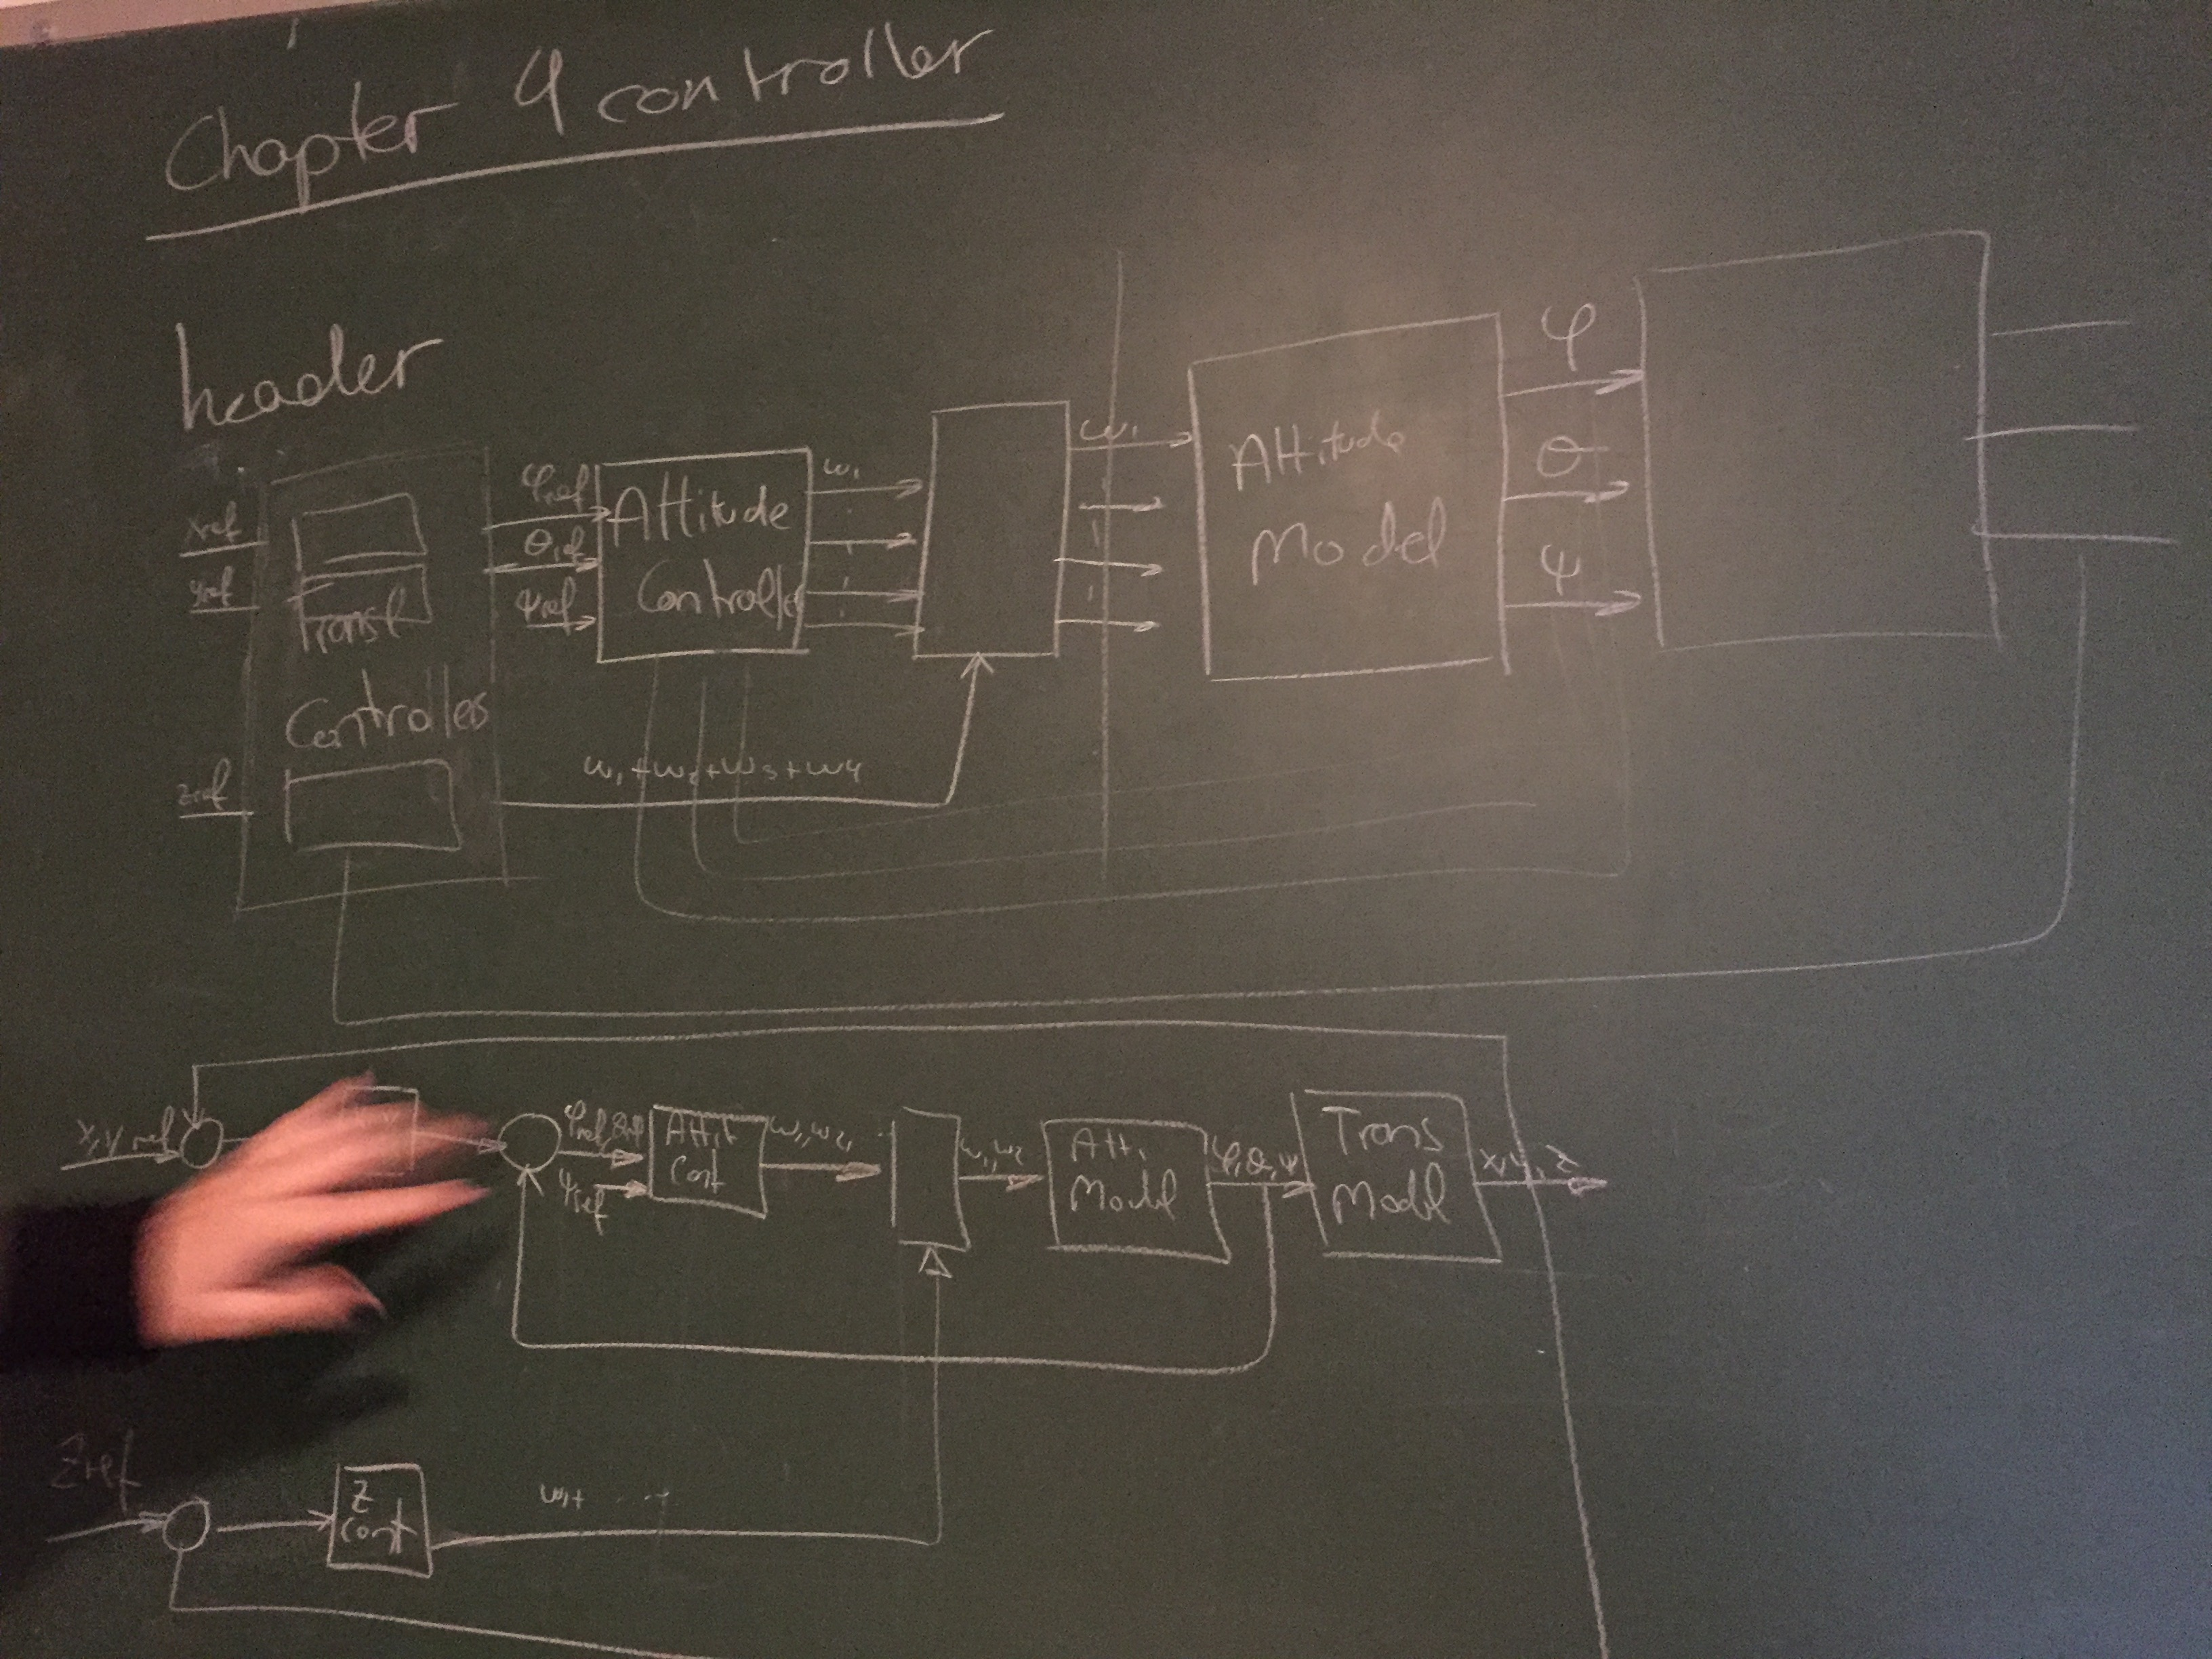
\includegraphics[width=0.7 \textwidth]{figures/ControlHeadDiagram.JPG}
	\caption{Block diagram of overall control system.}
	\label{fig:ControlHeadDiagram}
\end{figure}


\autoref{fig:ControlHeadDiagram} is a block diagram of the overall control system.
The attitude controller is an inner controller and is designed as state space, as this allows multiple inputs. The three angles roll, pitch and yaw are coupled and therefore complex to control individually, as the single controllers will disturb each other resulting in a less effective control system. The translational control system is going to be designed with classical control principles, where bode plots and root locus are the design method to obtain proportional controllers. 

First the design of the attitude controller is done followed by the design of the translational controller. 
When the controllers are designed, they are simulated with the linear models to ensure, that the controllers yield the desired behavior. Afterwards the controllers are simulated with the models, that are not linearized, as these represent the true behavior of the plant. If the controllers yield an acceptable outcome, they are to be implemented in the system. To do so, they are first discretized. It is necessary to simulate the discrete controllers and compare the results with the continuous controllers, as some design considerations may be lost in the discretization. Lastly the controllers are implemented on the micro controller and the system is to be tested in the Vicon room. 